\documentclass[10pt,twocolumn]{article}
\usepackage{oxycomps}
\usepackage{hanging}
\usepackage [english]{babel}
\usepackage [autostyle, english = american]{csquotes}
\MakeOuterQuote{"}
\pdfinfo{
    /Title (Set the Stage: Building an Intuitive Set Design Program for Amateur Creatives in Theatre)
    /Author (Bryanna Hernandez)
}
\title{Set the Stage: Building an Intuitive Set Design Program for Amateur Creatives in Theatre}
\author{Bryanna Hernandez}
\affiliation{Occidental College}
\email{bhernandez2@oxy.edu}

\begin{document}

\maketitle

\section{Problem Statement}
In stage productions and on-screen, a set designer is one of the unsung heroes of the visual medium. A set designer is responsible for bringing an environment to life while also embodying certain metaphorical themes like a character's journey. Using tools like scenery, the fixed backdrop of a stage, and set dressing, typically the decoration and furniture, set designers are responsible for modeling immersive scenes that are visually interesting and informative. Usually, a designer's creative vision is formed within their mind, but bridging this initial draft to the final product requires outlining, modeling, and refining a stage so it can be thoroughly communicated to the director, producers, and technical cast in charge of building the stage. For industry professionals, there are a variety of online tools that allow them to create in-depth and painstakingly detailed sets that productions can then spend thousands of dollars to realize. 

However, for smaller community theatres and public school productions, these online tools are extremely complex, typically repurposed architectural programs that require hours of tutorials and practice just to learn which tools are relevant and useful to their purpose. Additionally, many of them are expensive and require money that could be more thriftily spent on the stage itself. In order to address this need, I built a small-scale set designing program that is appropriate for amateur and low-complexity productions. For my project, the aim was to streamline the visualization process for these amateur set designers and create a final project that is simple, intuitive, and practical to use.

\section{Prior Work}
\subsection{Industry Tools}
The three primary tools used by industry professionals are SketchUp, AutoCAD, and Vectorworks. All three are self-described 2D drafting and 3D modeling software. SketchUp includes a "Push and Pull" functionality that allows users to extrude flat surfaces into 3D shapes. It also includes drawing layout functionality and surface rendering. Vectorworks allows paper and pencil sketches to be imported into Vectorworks using a similar Push/Pull command to create a basis for the project, and it uses a hybrid 2D/3D environment to see the direct impact of a 2D change on the 3D representation and vice versa. AutoCAD uses vector images and/or bitmaps and is designed for more architectural needs of plans and structures. 

In terms of graphical user interfaces, all 3 applications have similar methods of dividing the screen into multiple sections, with a graphical representation in the center surrounded by toolbars. The SketchUp web-based application confronts first-time users with a toolbar on the left-hand side that allows users to start creating a model with a pencil tool to draw lines, an arc tool to make circles, and a square tool. Users can also import models that have been created by other users through an incorporated search engine. AutoCAD is divided into a Graphic Area, where users can make their designs; an Options Ribbon that has the most common actions; a pull-down menu bar with tool boxes; a Status bar that gives information about coordinates and grid control buttons in vector form; and a command line. Vectorworks has palettes, and small windows containing tools that allow you to draw and edit objects. Upon first usage, palettes are hidden so users can customize their space with the most useful tools. Palettes include "snapping" which allows you to snap objects onto a grid; "attributes" which decides the color, weight, and fill of an object or line; "basic" which is used for drawing; and "tool set" with 12 sub-sections for specific tasks like creating a staircase.

When breaking down these three primary applications, it is obvious that the biggest emphasis has been to create a workstation that allows users to create custom builds by drawing or sculpting their own models from scratch. For the sake of time, I plan to focus more on developing software for visualization purposes over from-scratch creation. By providing a standard library of pre-created props and with basic lighting customization, I am lessening the number of extraneous tools within my program, simplifying it down to its basest needs. Because my targeted audience has simpler needs, it will be less necessary to create highly detailed and customized designs, and the focus will be on creating an easy space for amateur designers to place and evaluate their scenes.

\subsection{Building over Creating}
When switching to tools that are more similar to my focus, I have highlighted The Sims 4 and Virtual Architect Home Design Software (VAHDS). The Sims 4 contains a build mode that can be used to edit a lot's architecture and construction while adding, moving, and manipulating objects on a grid system, the view of which can be toggled. It contains a build mode tool menu that can move, resize, and delete objects; a design tool that changes the object's color or pattern; and a "Save To My Library" tool among others. It includes a catalog with objects sorted based on rooms that it would appear in, including Kitchen, Bathroom, Living Room, and Study. It can also sort objects by type, including surfaces such as tables and counters and decorations such as paintings and posters. It also has catalogs for roofing, windows, doors, and columns. Objects are shown in a list as small 3D objects with text description upon mouse overlay, and dropping them onto the grid demonstrates the number of square spaces they take up, in a fully 3D visualization. 

On the other hand, the VAHDS design system takes a top-down approach when it comes to adding walls and objects, choosing to specify measurements, angles, and lengths, rather than providing a grid system. The top of the interface contains a toolbar separated by Building, Interiors, Landscape, Terrain, Analyze, and Help. Within these categories, there are different subcategories of icons that will lead to a right-hand toolbar catalog, from which items can be dragged and dropped onto the screen, rendering in a simplified 2D drawing. A selected item will be displayed in the bottom right corner with its rendered 3D model in more detail. A bottom toolbar has more general tools like zooming in and out, rotation, and changing floor plans. Outside of its top-down view, cameras can be inserted inside the house with viewpoints on a swivel, so that users can see the 3D visualization. 

Unlike VAHDS, The Sims 4 has 360 camera rotation capabilities, with various camera controls for viewing the environment. Using the keyboard or a mouse allows users to zoom in or out; directional keys allow the user to move the camera; the shortcut "T" goes into a top-down view; and using a mouse allows the player to pitch or tilt the camera. Because of these controls, it does not contain any automatic isometric projections.

The Sims 4 is a video game built for entertainment value, and its build mode was created in mind for designing full buildings. It can fully render textures and lighting. Its ability to completely render a 3D model is more preferable to some of the other industry tools that requires secondary tools. However, its camera layout when building the model leaves something to be desired. I prefer to take inspiration from VAHDS' fully two-dimensional build mode that transitions that user into a three-dimensional viewing mode. However, instead of making the user place their own cameras, I decided to pre-program up to 5 different viewpoints based on the stage's dimensions that allow the user to see their model from an isometric view, as well as sample audience perspectives such as in the front row or on a balcony. Taking this extraneous control away from the viewer with further simplify the software, allowing users to focus on the design rather than camera controls. Additionally, I prefer to defer to VAHDS' system of displaying props in a 3D render in the corner of the screen, allowing users to preview the objects before placement. 

\subsection{Timeline Tools}
One last application I looked at was danceapp.us. While this tool is marketed for creating dancer formations, it has a wide range of applications in terms of blocking. Set designers are not necessarily expected to plan for stage directions within a script, it can be useful for the director and designer to collaborate and ensure their visions for the stage don't conflict before building the set. This application has a timeline on the bottom of the screen that allows users to specific which frame they are designing in. Adding a new frame and repositioning the dancers makes them automatically move when the animation is created. It is a simple but useful application, and I believe that this basic method for desiging a timeline keeps the interface intuitive while fulfilling its purpose. Integration of this functionality will help set designers to keep the purpose of the scene in mind and imagine ways that their scenery and staging can facilitate the play.  

\section{Technical Background}
\subsection{User Interface Design}
I am creating a brand new software which focuses on user interface design, referring to the front-end of software development. UI provides a platform for the human-computer interaction, and it is divided into Command Line Interface (CLI) and Graphical User Interface (CUI). CLI is text-based and refers to a set of instructions. In order to allow non-programming users to interact with the software, a GUI system is preferred. A GUI system includes the window, where the contents of the application are displayed; a menu, which is the array of standard commands grouped together in a visible place; an icon, a small picture represented an associated application; and a cursor for interactivity. It can also contain dialogue boxes, buttons, check-boxes, and sliders. GUI design should typically be consistent, allow for short cuts, offer simple error handling, permit easy reversal, and make users initiators rather than responders to the system. Within GUI Design and implementation, it is important to have various tests for usability, compatability, and user acceptance. 

\subsection{Object Modeling}
The main component of this project is related to computer graphics. Computer graphics includes object modeling, which is the computer rendering of geometric representation of objects. Rendering is the process of generating these images through light simulation, shading, color, texture, and related visual effects. It can also include animation, which is the changing of these objects that simulates an illusion of motion. For this project, I am not creating a rendering engine from scratch, but it is still important to understand how it works so it can be properly manipulated and to better understand time complexity of running a program. Rasterization is the process of projecting objects in a scene to an image plane. This means translating object surfaces, usually made up of multiple triangle meshes, usually in object order algorithms which are more efficient than image order algorithms which iterate over pixels.

Ray casting is the process of using geometric formulas to compute intersection, which can be useful for determing shadows or intersecting sightlines. Ray tracing simulates the bouncing of light paths caused by reflection and refraction, which requires various ray casting operations. Ray tracing can render effects like depth of field and blurriness, and it is most likely beyond the scope of this project. However, radiosity is an approach that breaks a scene into pieces and estimates the amount of light each piece gets, which is another method of rending shadows. 

 Real-time rendering, often used for video game graphics uses rasterization but combines it with ray tracing and path tracing. In order to make it occur in real-time, it often relies on pre-rendered lighting for stationary objects, and it uses light probes for moving objects. However, rendering is usually a tradeoff between speed and realism. In this project, speed is prioritized over realism.

\subsection{Isometric Projections}
When visualizing objects, there are different types of 3D projections. Orthographic projection is the easiest type because it ignores the z axis and project objects without considering depth. This type is not as useful for this project since a 3D stage necessarily implies depth. Another type is Perspective projection, which is similar to real world perception because it emphasizes vertices closer to the viewport by making them bigger. This projection is achieved through a perspective divide, by making the projected values of x and y inversely proportional to depth. The bigger the depth is, the smaller the resulting x and y are, so that things that are farther appear smaller.

Lastly, there is Isometric projection which visualizes 3D objects in two dimension, so that the x-axis, y-axis, and z-axis are equal to 120 degrees. This is a configuration of orthographic projection that ignores depth, and it is typically used to allow programmers and artists to create more elaborate environments. Isometric projections are often cheated by using 116.57 degrees for the x and y axes and 126.87 degrees for the z-axis, creating a 2:1 ratio that simplies trigonometric calculations and allows tiles to be 100x50, 600x300, or 64x32 evenly. This is a "pseudo" isometric angle that seems useful for a viewport angle and allows users to see their models from a dimetric lens that simulates depth.  

\section{Methods}
\subsection{Codesign Interviews}
As I am building this project for a very specific demographic, and I want to make sure that it meets their needs, I started the process by meeting up with a group of college theatre majors who were interested in physical set design . Understanding that this software could have various other uses, such as for writers or dancers, I also periodically held interviews with other non-theatre majors, such as computer science majors and other media majors. Throughout the semester, I sought out familiar as well as new participants to review my software in order to gain a wide range of feedback. 

For the first interview process, I made sure to ask the participants about their process and what features they felt would be the most useful. I had them outline the various ways that went about designing, and what types of scenes that they made most commonly. I also asked them to show me some of the past set designs that they have worked on to get a better idea about the complexity of their work. I asked many of them how much experience they seemed to have with using online 3D tools and almost none of the theatre majors confessed to having much experience with any of the above programs mentioned in prior work, aside from The Sims franchise. After this first stage to gain more information, I transitioned to outlining the features that I envisioned adding to the software and encouraged them to provide detailed feedback about their thoughts and if they felt that my software was missing any features, of which I gained various feedback regarding the amount of control and complexity available to them. 

After completing a landmark feature of the process, of which the features will be further outlined below, I conducted interviews in order to determine if the user interface was sufficiently intuitive for users. As the program became more complex, these interviews become progressively longer, and I started to test users on their ability to utilize the software in order to create basic scenes. This process was mostly hands-off in terms of explaining the interface, as I made sure to take notes on how users interacted with the program and what issues they came across organically. While I also asked for their feedback afterwards, I found that they were typically more involved in trying to offer extraneous feedback about new features they would like, so I felt that the most useful feedback was found through my examinations of their work. The changes that I made due to these sessions will be pointed out in the appropriate sections below. 

\subsection{Navigating a 3D Space}
As I discovered that many of my prospective users were unfamiliar with navigating a 3D space, I decided to tackle this issue by creating a camera menu that allowed users to toggle between labeled cameras. I chose five camera views based on the codesign interviews in order to cater to the angles that were most valued. These camera views were as follows: a top-down view, a straight-on forward view, a slightly angled forward view to simulate the angle of the audience, an isometric view from the left side of the audience that prioritized the left side of the stage, and an isometric view from the right side of the audience to prioritize the right side of the stage. In addition to these five views, I added a sixth split-screen option that allows users to view the first, third, fourth, and fifth camera angle at once. It quickly became apparent that it was essential to label the camera views in the split-screen to prioritize comprehension.

Additionally, in order to further acquaint users with the layout of the scene, I made sure to add a backdrop and wings on either side of the stage, simulating the set-up of a real proscenium stage. In order to allow users the maximum view of their designs, I also included a botton to toggle the menus, getting rid of or bringing back all other UI. 
\subsection{Straightforward Customization}
In order to allow users to opportunity to build scenes without having to create props themselves, I created a simple prop menu. In this prop menu, filled with assets found from the Unity Asset Store, I assigned each asset to a labeled button. In order to maximize menu space, the button only have text, but when they click on a button, it allows them to view the prop in a side camera. This is to prevent users from accidentally adding props to the scene and having difficulty organizing their sets. After viewing the prop in the side camera, users click a button to add the prop to the set.

As part of the feedback from the codesign process, I added a feature that assigned each prop to a category such as "Park" or "Furniture" allowing for further ease of navigation of the prop menu. If users decide that they only want props that would fit in a park scene, they can deselect any unrelated buttons at the top of the prop menu, and they will only be exposed to props that fit within the park category. 

Once a prop is added to the scene, users have further access to customization options. When users hover of the object in their scene, the object's mesh outline becomes highlighted, allowing users to understand which object they are about to select. Once the select the object by clicking on it, a new menu appears, connected to the prop's properties. In this menu, specific to the props, users are able to adjust the X, Y, and Z coordinates of the object, as well as the size, and the rotation of the object on the Y axis. These 5 options can be adjusted using a slider that gives real-time feedback to the user. Additionally, there is a deletion option attached to this menu, that allows users to get rid of the object in the scene. If users get rid of the object, a second "undo deletion" button will appear on screen, giving them the option to either bring the object back into the scene, keeping the same properties it had when it was deleted, or get rid of this option by selecting the red "x" button. This undo button only works on the most recent deletion, but through user testing, I was able to verify the userfulness of this features for users who were debating the effectiveness of an object in the scene. 

As part of this section, I also included two types of lighting options that users can add to enhance their scene. Based on the vocabulary of the theatre students, I termed these lights as "point lights" and "floodlights," and these lights also come with their own unique customization menus. The first type of lighting, floodlighting, is derived from Unity's pre-existing lighting feature, directional lighting, and essentially acts as the Sun in a scene. It is a light that spans almost the entirety of the stage. While users are unable to click on this light directly, I included a separate button that allows users to access the floodlight menu when they want. Included on this menu is the option of changing the R, G, and B values of the light, the intensity, and the X and Y rotation of the light through changing real-time sliders.  

For the point lights, users are able to access them individually through clicking when they add them to the screen. Taken from Unity's pre-existing point lights, I created a prefab by attaching a sphere to the point light, making the physical object easy to spot. When users hover over these lights, the sphere mesh outlines are highlighted in the manner that props become highlighted, giving users further information on what they are able to select. When the point light is selected, users have the options to customize the color throught its R, G, and B values, the intensity, the range, and the X, Y, and Z coordinates. While point lights are intended to be focalized sources of light, the range property allows users to use a point light in a similar manner to the floodlight if they so choose, allowing them to choose between which type of light they prefer to use. However, users often employed the point light for light sources such as a street lamp, or to provide varied colorful lighting.  

Through my codesign session, I came to understand that many users became frustrated with the inability to directly select the floodlighting that they added to the scene, especially after adding other types of lights. In order to provide an easier fix, I additionally added a reset lighting button that gets rid of all lighting within the scene, so that users are able to start over and reapproach the lighting of the scene without feeling like they have lost control over the creative process. 
\subsection{Saving and Timeline Animations}
While creating a scene is an important aspect of set design, the process of set designing typically ranges over a multiple-scene production. Therefore, I added a feature that allows users to save and load the scenes that they had built. By using a slider in the top left corner, users are able to determine for themselves what scene they are in, for example in the second scene. Once they are satisfied with the creation of the scene, they can save the scene, and the properties of all the props and lighting features will be saved to a specially-reserved layer for that scene. Users are then able to make changes to the scene, change which scene number they are, and save a new scene, without making changes to any of the scenes that they have previously saved.

When users want to load scenes that they have already viewed, they can move the slider to the number they wish to see, and press the "load" button. This completely erases the current scene, and loads in all of the props and lighting features associated with this specific scene number into the user's view. If a user makes changes to a loaded scene, they must save these changes once more in order for the program to understand their changes. 

Additionally, there is an animation feature that allows users to view all of the scenes that they have viewed in order under the "Animation" menu. When users load in this menu, they will see options to adjust the time, in seconds, of how long they want each scene to appear on stage. When they adjust the metrics to their liking, they can press the bright red "Play" button, and their scenes will load-in order for the number of seconds they have requested. The transitions between these scenes are discrete, without changes in the positioning of the props or lighting features. Essentially, this feature is the same as loading in all the scenes in order, but it automatically toggles off the menus and allows users to spend more time viewing their scenes through automatic transitions, instead of focusing on changing the scenes themselves.  
\section{Evaluation Metrics}
In order to evaluate if the problem I set out to the address has been solved, I utilized certain metrics in the final interviews of my codesign process to evaluate the satisfaction of the user experience. While the in-between interviews were good benchmarks to understand general satisfaction with the features throughout the process, I used these final interviews to gain information on satisfaction on the features separately and as a whole product. 

The evaluation metrics are both qualitative and quantitative in measure. The first test I did was an observation test, asking users who had been part of my process, as well as new users, to sit down with the software and attempt to make a specific scene within a certain time limit. This test was used to evaluate how quickly users were able to pick-up the initial features of the camera angles, and the prop and lighting libraries. By instituting a time limit of 15 minutes, based on the somewhat small prop library and the basic requirements for creating a scene, including four relevant props and adding in one light source, I evaluated the users on how intuitively they used the program without my intervention, including how often they decided to change camera angles and how easily they were able to navigate the prop library.

Next, I asked users to save their initial scene and create a second scene based on their own creative sensibilities. This creativity-based test allowed me to better understand how users naturally consider the program in their creative workflow, as opposed to using it to complete a more specific task. Included in this test was an evaluation of how long users spent creating, and whether this amount of time was based on a consistent creative workflow, or if users felt stumped or blocked in their creative process. Again, I did not intervene in this test, except to confirm when users had satisfactorily finished and saved their scene.

Lastly, I tasked users with playing the animation of their two scenes, seeing how long it took for users to grasp how to utilize the timeline and adjust the number of seconds on the screen to their liking. 

After this set of observation tests, I engaged users in a survey to understand their subjective understandings and satisfaction in using the product. These questions asked users to: rate their satisfaction from 1-10 with the product in general, rate the different features (camera toggles, prop library, lighting features, and save/load features) from 1-10 alongside targeted questions on what they found to be the easiest or hardest part of the feature to use. I also asked users to detail how they could imagine using the product in their creative workflow in the future, if they felt that they would realistically ever use the software again, and any final miscellaneous feedback they wanted to give me. By mixing up the survey with multiple choice questions and short answer questions, I was able to gain a better understanding of how users viewed the product in their own words, and whether they would rate their satisfaction highly (above 7 on the scale), moderately (between 4 and 6), or lowly (below 4 on the scale). 
\section{Results and Discussion}
Starting from the quantitative results of the surveys, the average rating for the product in general, from a mixed group of theatre major and other types of college students, is rounded to an 8.6. Separating these groups by majors, it is evident that the average of the overall rating of theatre majors was 8.25 compared to a general average of 9.1 for non-theatre majors. From this ranking alone, it is a quick measurement to see that the satisfaction with the software can be ranked highly. However, going deeper into the qualitative tests as well as the feedback reveals some of the dissatisfactions with the product that would need to be addressed in order for more users to feel comfortable bringing this into their workflow.

Regarding the observation tests, all observed users were able to complete a scene of 4 props and a light source in under 5 minutes of initial contact with the software. This demonstrates to me that the overall user interface layout is extremely intuitive to use and takes almost no time at all to understand the mechanics of the design, a key aspect of some of the other industry tools that I hoped to improve upon. During the more creative portion of the observation test, users were much more active in interacting with object properties and changing the camera angles to better suit their visual needs. While I noticed a general frustration of some users, specifically non-theatre majors, wishing that they had the ability to use keyboard shortcuts as a way to change the camera angles, I noticed that all camera angles except the forward "audience angle" were commonly utilized, and users had little to no issues in selecting objects. Additionally, some of these same users expected to see a similar UI such as in 3D programs like Blender or Unity which allows you to move an object by dragging. However, they were quickly able to adapt once they discovered the object properties menu. When there were overlaps in selection that prevented them from selecting the object they wanted, they realized quickly that the best solution was to spread out the objects on the stage first before placing objects. Additionally, categorization was used by all users in this portion, as they used the limitations of the categories to decide on the exact circumstances of the scene they wished to portray. A majority of all users chose to use the park props over the furniture props due to a wider range of options and many users also placed characters within their scenes. 

The biggest discomfort that I observed during these sections was the continued frustration with the floodlighting, based on a lack of cohesiveness. With the other props and the point lighting, users are easily able to hover over and select objects. However, many users realized that it was difficult to add multiple floodlights and change their settings in retrospect, and I noticed many of them making the switch to exclusively using point lights with a larger range as a replacement. This frustration was more commonly shared between theatre major students, who in general placed a more specific interest in lighting than the non-theatre major students. 

There was a short adjustment period for users to understand saving and loading scenes, as they initially understood the timeline between these two buttons as communicating the current scene layer that the props were on, and not understanding that they had to save the scene first. However, after this first mistake in saving, almost all users were able to change their understanding of the UI. Once the saving button was fully comprehended, users had no difficulty in understanding how to load scenes. This misunderstanding was shared between both groups. 

Additionally, I observed no difficulties in users in their initial understandings of the animation timeline from either set of students. Users were able to use the sliders without difficulty to change the number of seconds a scene appeared, and were able to understand that the animation had started easily due to the disappearance of the animation menu. 

Taking this into account with the rest of the survey questions, it comes to no surprise to me that feature of the camera toggles was the highest rated feature with an average of both groups of 9.3 out of 10. While some of the non-theatre majors expressed a wish to have more control over the angles, all users felt that they were able to accurately place and understand the depth of the stage based on the variety of angles offered and the context clues of the stage features provided. Some noted that the stage certainly seemed much smaller in certain angles such as the forward view, but that this was rectified in the top-down views and the isometric views. 

As for the prop library, this feature was rated at a high satisfaction of 8.7 out of 10. The most common complaint was a lack of robust options for creating diverse scenes, which I consider to be an overall limitation of this software, most users reported satisfaction in the ability to see the objects they had selected. Many acknowledged that they liked the usage of sliders, specifically the X coordinate, since it matched the visualization of the prop moving on stage. Users also expressed that the ability to change the size of the object was useful, but that it was sometimes difficult for them to gauge the correct scale due to many of the objects coming from different packs and having slightly different starting dimensions. Overall, many users decided that they felt the prop library was built in such a way that they were quickly able to make decisions on what to add to their scene. 

The rating for the lighting features was the lowest ranked, dipping into a medium satisfaction rating of 7.4 due to the general frustrations with the floodlight menu. While many of the users decided that the features of the point light was enough to make up for the shortcomings of the floodlights, and that they were able to express a range of lighting options with the ability to change color and size of the point light, most of the users complained that the floodlighting made the initial exploration process more frustrating. Due to this, it does seem worth considering an overhaul of the construction of the floodlight or getting rid of it entirely in order to increase user satisfaction to a high level.

Finally, the saving/loading features had a high satisfaction score of 8.2 out of 10. Despite the initial confusion reported above that many users had with the system, most of them reported that they were satisfied with the functionality of the saving and loading features, such that it allowed them to functionally reload the scene if they made changes that they didn't like to the scene. Grouping this section with the animation timeline, many non-theatre majors remarked that they didn't see themselves using the animation timeline often due to it having a somewhat repetitive function to saving and loading, but that they felt the feature worked intuitively and as it should. From this, I can see that it isn't necessarily a detracting feature, but perhaps out of the scope of interest for this section of the participants. On the other hand, a few users suggested that having the option to switch between continuous or discrete scenes might be using for scenes that utilize the same props with a few adjustments in positioning. 

For the relevant users, it was a mixed group of users saying whether they felt the software would be suitable to add to their workflow. A few agreed that it could be useful, with the caveat that its current state of props would be lacking for a wide variety of productions like fantasy or Shakespeare productions. I additionally had a few users state that they would love to use this software outside of set designing prospects, such as designing a scene as a writing reference. Most participants agreed that they would be interested in trying out the software in the future, to see what other kinds of combinations of scenes they could create, once more stating that the number of scenes they would be able to create is a bit limited. 

Based on this variety of feedback, and taking into consideration one of my main goals of creating a software that could be beneficial to set designers, I would conclude that the overall high satisfaction with the product's features and how they work means that I have the framework for a software that could be improved upon in the future to be released as a more robust set designing tool. Combatting specific issues related to lighting or updating the animation timeline for a higher variety of uses also seem like beneficial ventures, but overall, I feel satisfied in saying that the software is a useful and intuitive product with large potential and would be definitely be useful for set designers if it were to be released to the public. 
\section{Ethical Considerations}
\subsection{Technological Solutionism}
Technological Solutionism is essentially the arrogance of believing that every problem in our society has a solution if only one can create the right algorithm. As the creator of this term, Evgeny Morozov, acknowledges in an interview with Natasha Dow Schüll that the issue doesn't come from utilizing technology as a new part of our "problem-solving apparatus". Instead, the issues lie in the pursuit of reducing complex problems down to the numbers without "any holistic understanding"(Dow Schull). This results in a problematic understanding of a situation with a single, uniform solution for all people without considering the inherent diversity of their needs.

In the practice of using computer science to provide a creative tool, it is therefore imperative to ensure that the software doesn't force its users to conform to a singular practice or attitude regarding creative expression. Edwin Creely and Danah Henriksen's paper \textit(Creativity and Digital Technologies) examines the role and advantages of digital tools, positing that they provide safe spaces for "managed risk-taking and enacting constructive failure"(Creely and Henriksen). For my project, this is most relevant when considering the lack of physical costs regarding creative risks, as the software allows for an in-between stage between inception and material realization. 

However, the software is only suitable for a limited use of experimentation. In the supposition that creativity requires a sufficient balance of "embodied play, touch, and interpersonal interactions" my project would be unable to satisfy those requirements(Creely and Henriksen). Starting with the idea of embodied play which requires a tangible usage of the corporeal body, interaction through a digital screen would at best be able to simulate physical connection through haptic controllers such as the Playstation Five controller, which vibrates and responds to player breath in certain situations. This type of haptic interaction is completely beyond the scope of my project as it can only be used through a computer with a mouse. As an extension of this subject, the visual nature of software faces issues of accessibility for blind or low-vision individuals.
\subsection{Lack of Diverse Representation}
In scavenging the Unity Asset Store for appropriate props to add to the library, I selected an asset pack that included a cast of human characters for users to move as props. However, all of the characters are white, light-haired men and women, adding to a persistant pattern of a lack of diverse representation within both the computer science and theatre industries. Representation and diversity is an ethical issue as it relates to the acknowledgement of "the dignity and unique contributions each person" can offer (Kittner), ensuring that each person is given equal respect and rights. By choosing the settle for a cast of heteronormative characters without any noticeably black, asian, hispanic, etc. characteristics, it feeds into a history of exclusion of the basis of appearance rather than personality and achievement. 

While the scope of this software as a demo necessarily limits the amount of props and characters that can be added, as well as the semester time crunch and the lack of resources with which to purchase more diverse assets, it is regrettable that I have had to trade inclusion for efficiency, and I want to use this section to acknowledge the potential impact that may have on my userbase, perpetuating the notion that there is a certain kind of person who deserves to exist in theatrical or technical spaces. While I was able to add a wooden mannequin that acts as a neutral middle ground, taking race and gender out of the equation, I would encourage users to carefully consider the situations and combination of usages of the characters and the mannequin to resist further perpetuation of discrimination and stereotypes within their fields and the world at-large. 

\section{Appendix}
\subsection{Replication Instructions}
For this project, the software was built in Unity Editor ver 2021.3.11f1. For coding scripts, this was done in Visual Studio Code, and the props in the library were downloaded from the Unity Asset Stores. The specific packs are included in the GitHub repository. 

In order to run this program, download the folder in the GitHub repository 
github.com/bry693/CS(underscore)Comps
(underscore)2024/tree/main/SetDesign/ 
and run the application SetDesign.exe found in the Logs folder. Otherwise, use this repository to open the project in the Unity Editor to view the project code. Note that the (underscores) must be replaced for the link to work. 

\subsection{Code Architecture Overview}
The code was organized into C sharp scripts using Unity libraries. In alphabetical order, the first script, AnimationPlay.cs uses the user's input from the slider of how long the animation should be and loads the scenes in order according to these values, clearing out the scene between loads. NewProp.cs is used to delete props from their parent, moving them to a different parent holder and adjusting the values of the prop menu sliders to adjust to the first child of the parent which is used to keep track of all the props. OnMouseDown.cs is used to select props and move their position of the parent so that the property menu sliders match the properties of the selected object. OutlineSelection.cs is used to highlight the mesh outline of an object with the mouse over it. ReadInput.cs and ReadLightInput.cs update the properties of the first child of the sceneparent and lightholders parent to match the values of the sliders in their menu object properties. Spawner.cs spawns a prop to be viewed before it can be added to scene. SpawnToScene.cs adds a prop to the scene under the sceneparent while SpawnLight.cs adds the light object to the scene under the lightholder parent. Finally, TimelineSaving.cs saves the current props and lights on scene to the associated layer of the selected scene number so that it can be loaded back into the scene later. The program is further organized into 4 canvas menu screens, which function according to the code architecture detailed above in the methods section. 

\section{Images of Software}
\begin{figure}[t]
    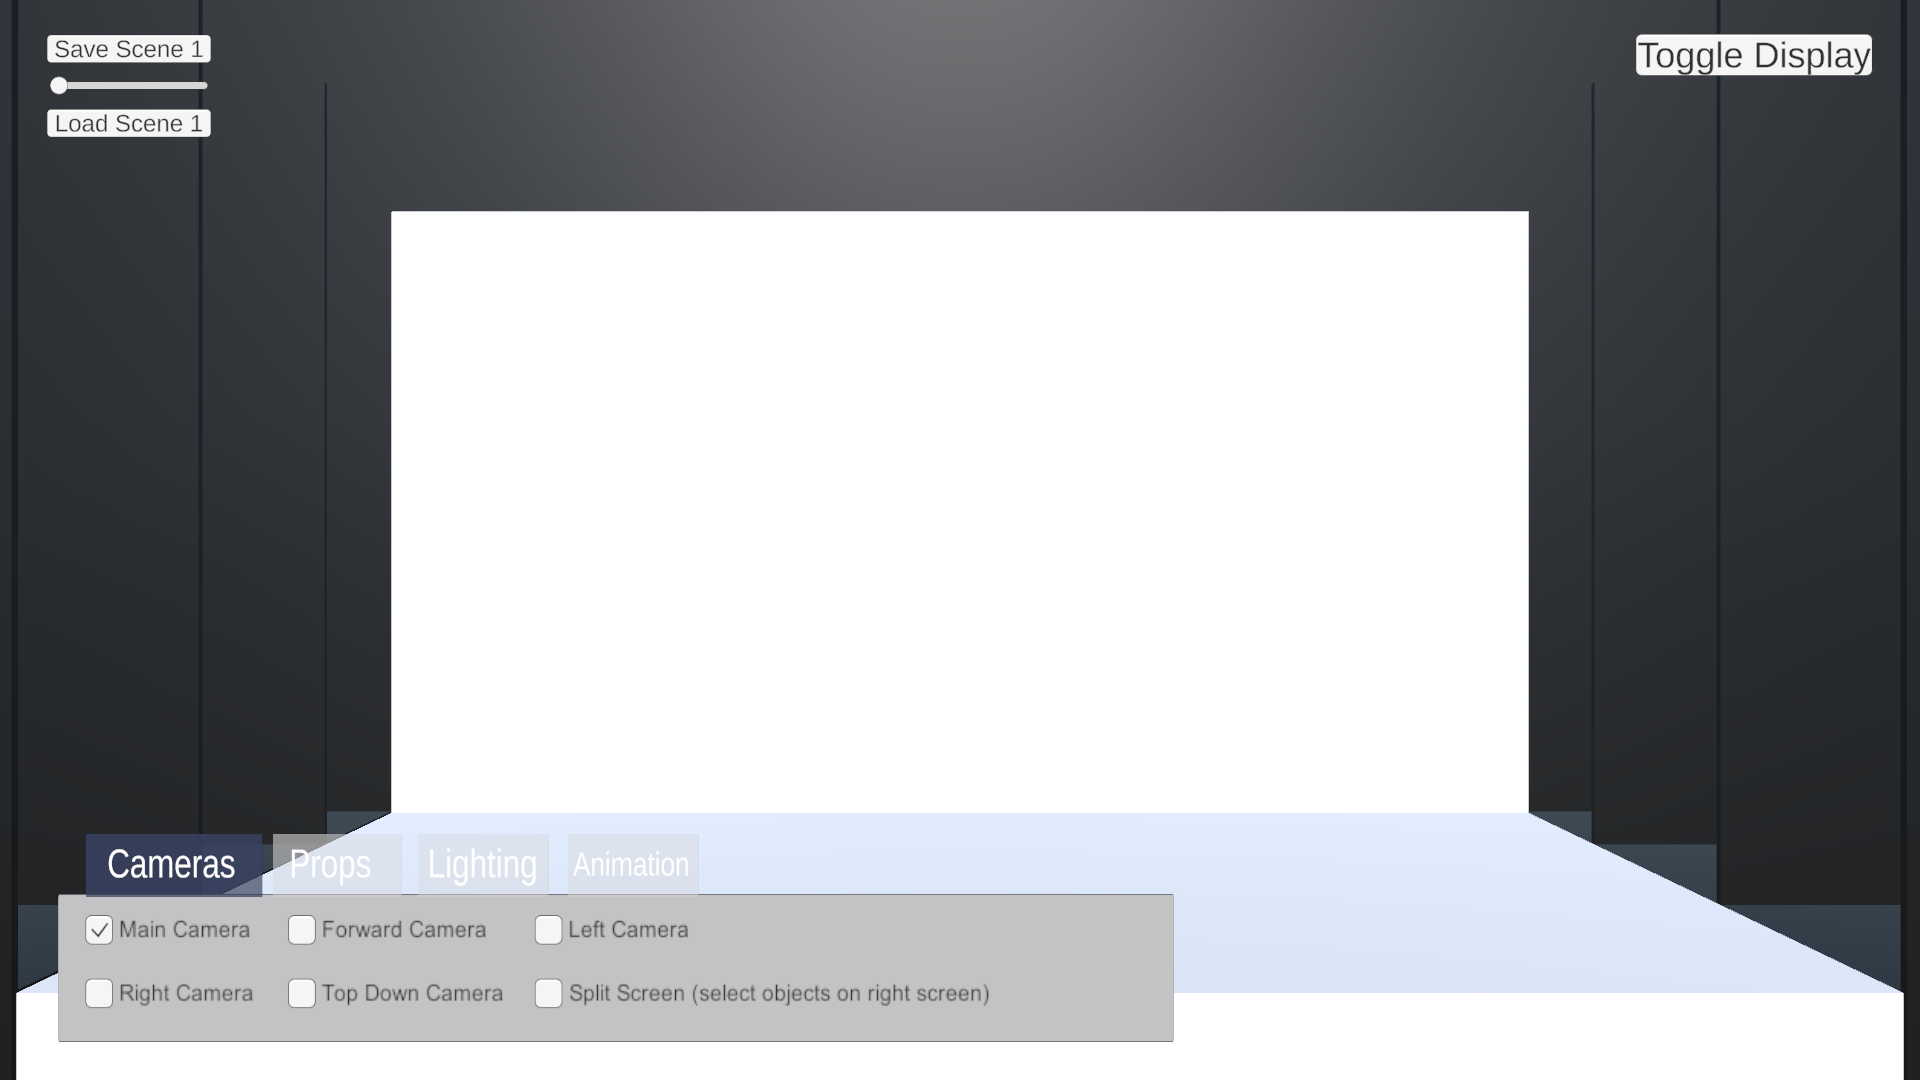
\includegraphics[width=.75\linewidth]{blankcameras.png}
\centering    
\caption{
        Opening screen with the default view and the variety of camera toggles.
    }
    \label{fig:Fig1}
\end{figure}

\begin{figure}
    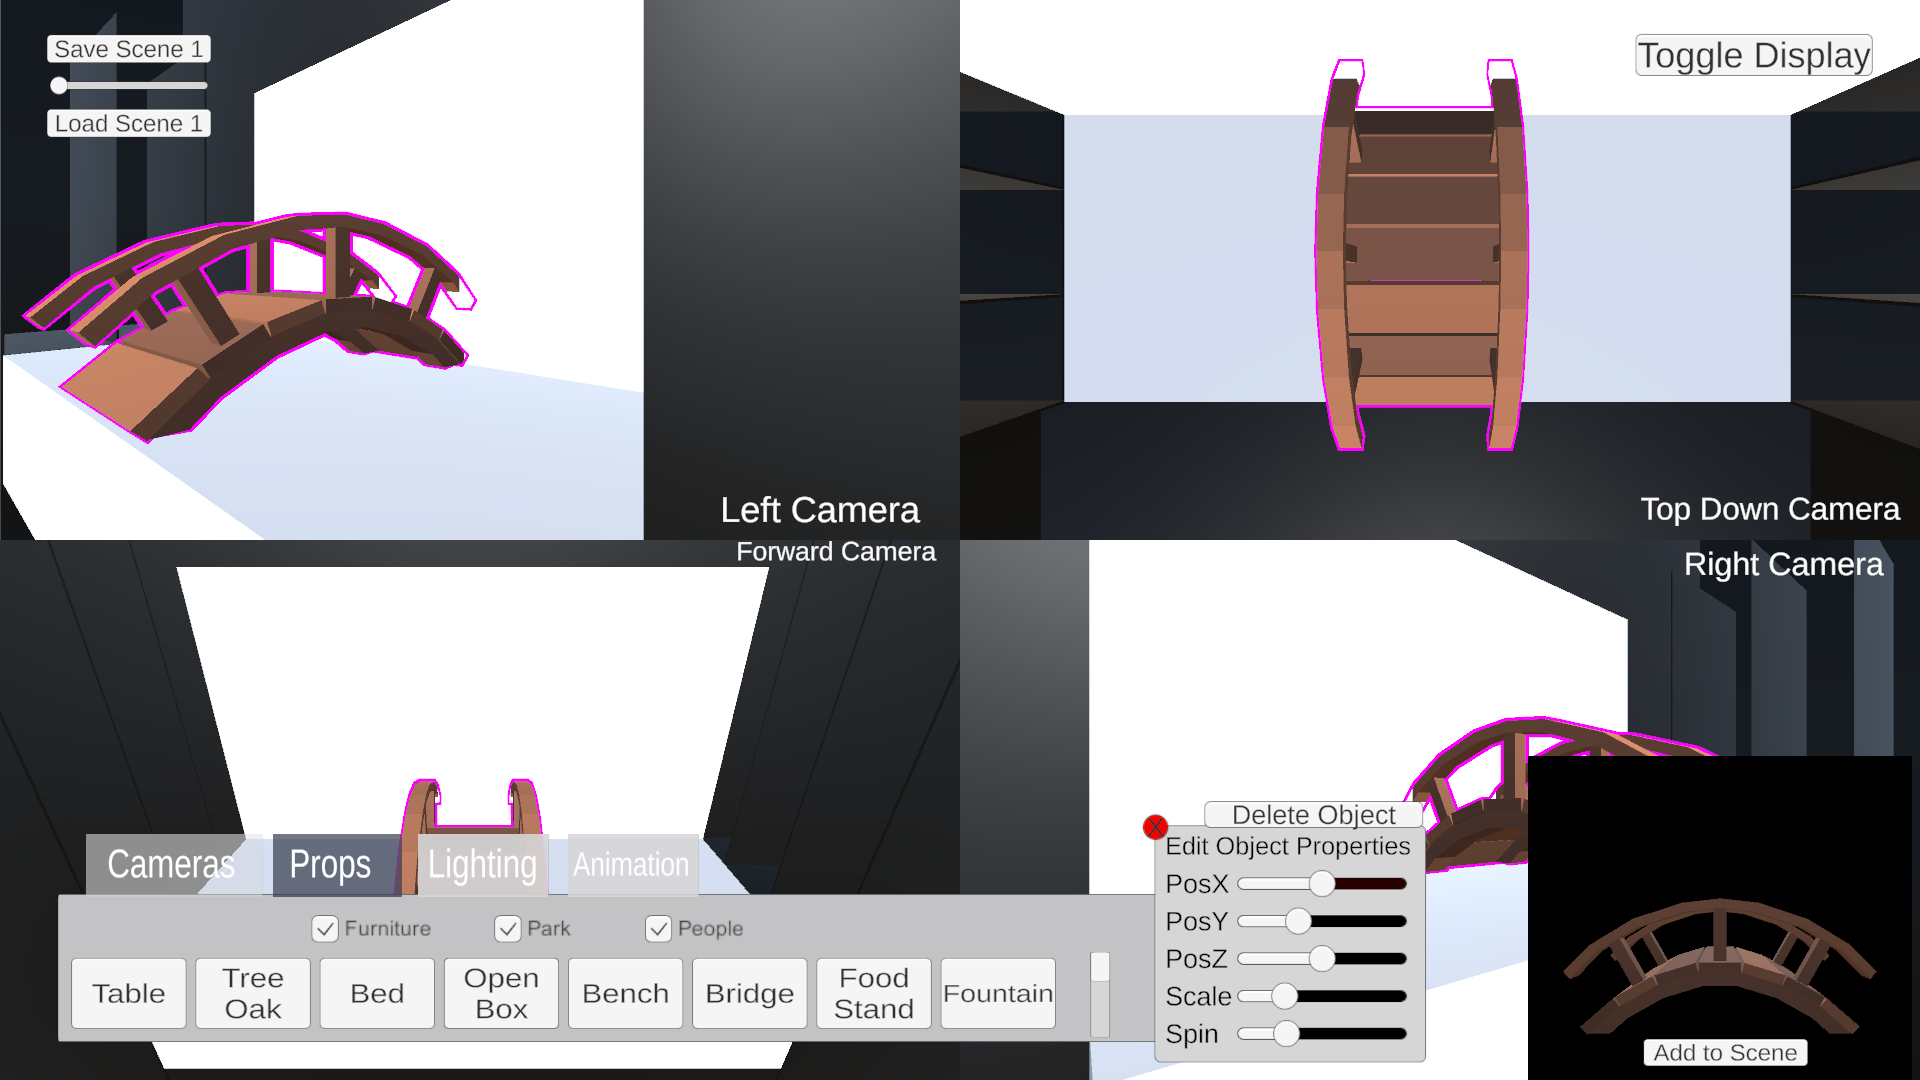
\includegraphics[width=.75\linewidth]{addbridge.png}
\centering
    \caption{
        View of adding a prop in split screen camera mode with property menu in view. 
    }
    \label{fig:Fig2}
\end{figure}

\begin{figure}
    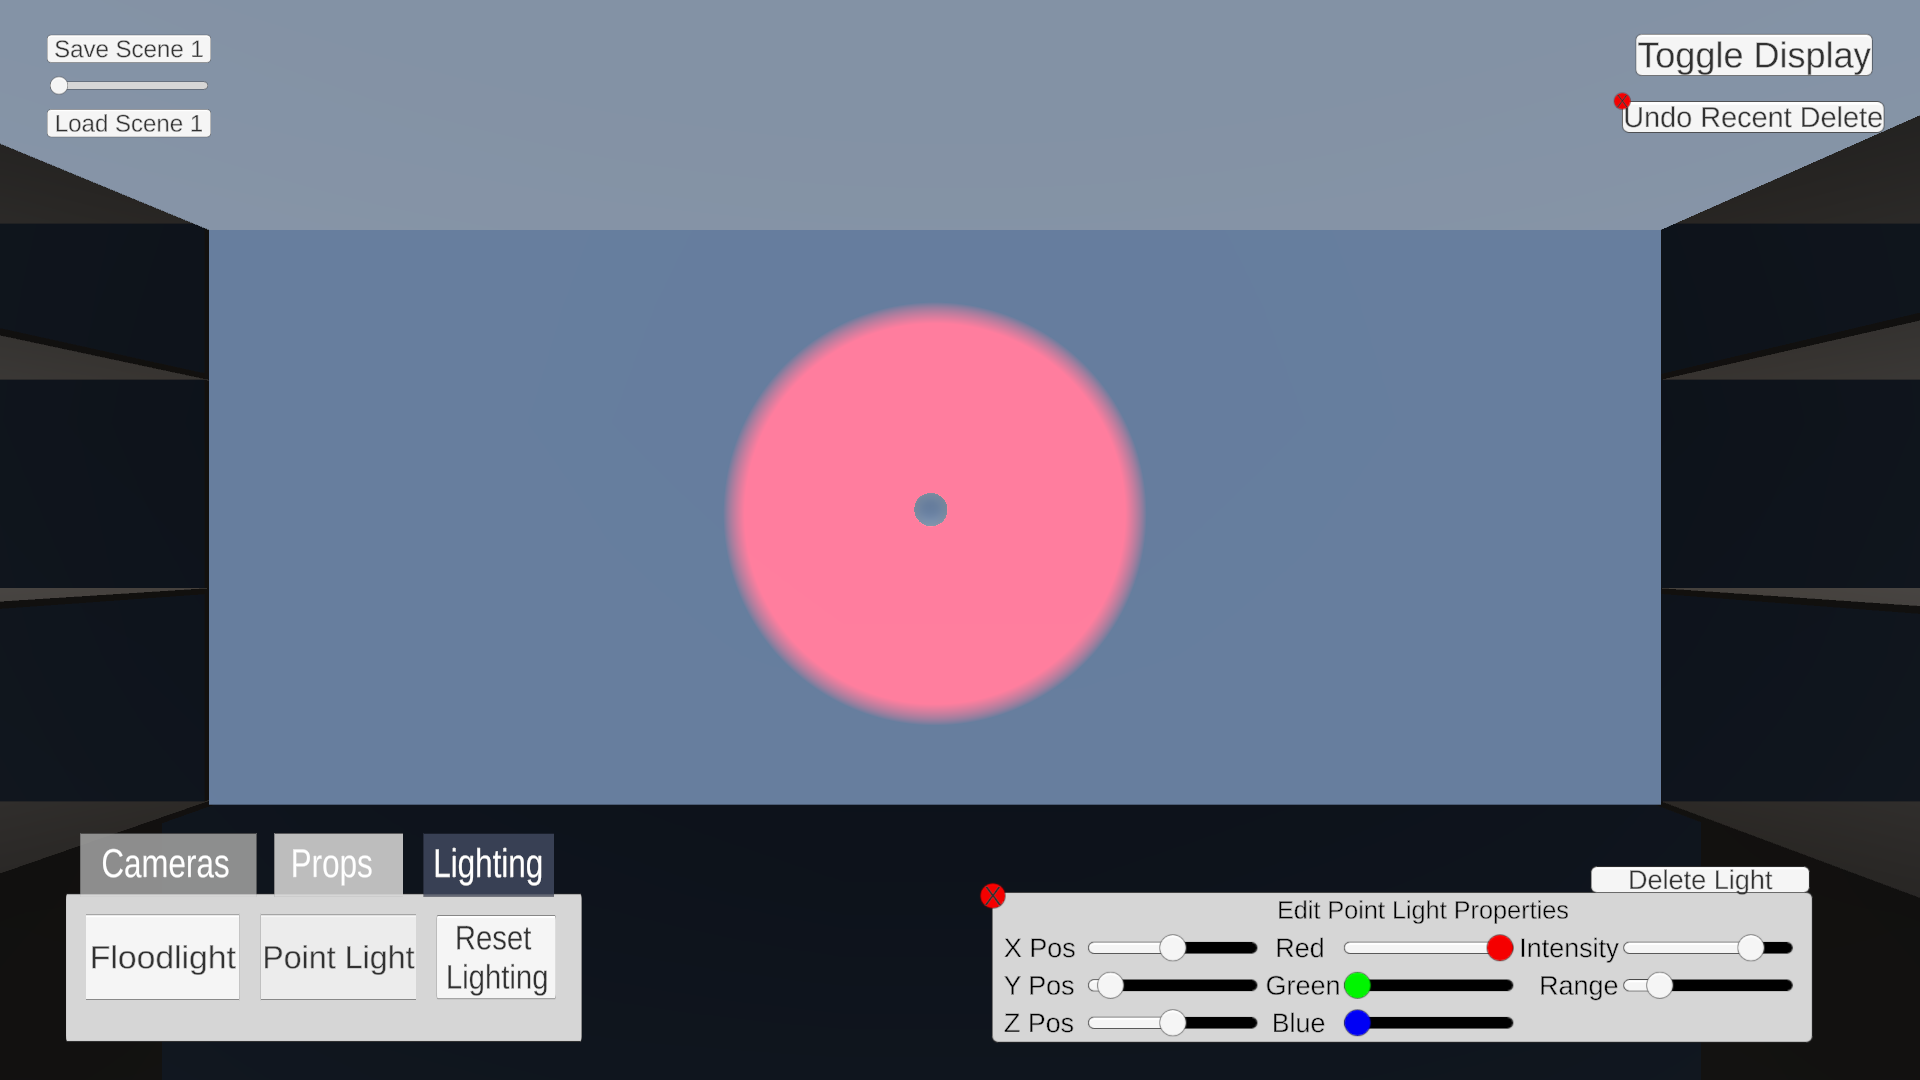
\includegraphics[width=.75\linewidth]{addlight.png}
\centering
    \caption{
        View of adding a point light with the associated menu.
    }
    \label{fig:Fig3}
\end{figure}

\begin{figure}
    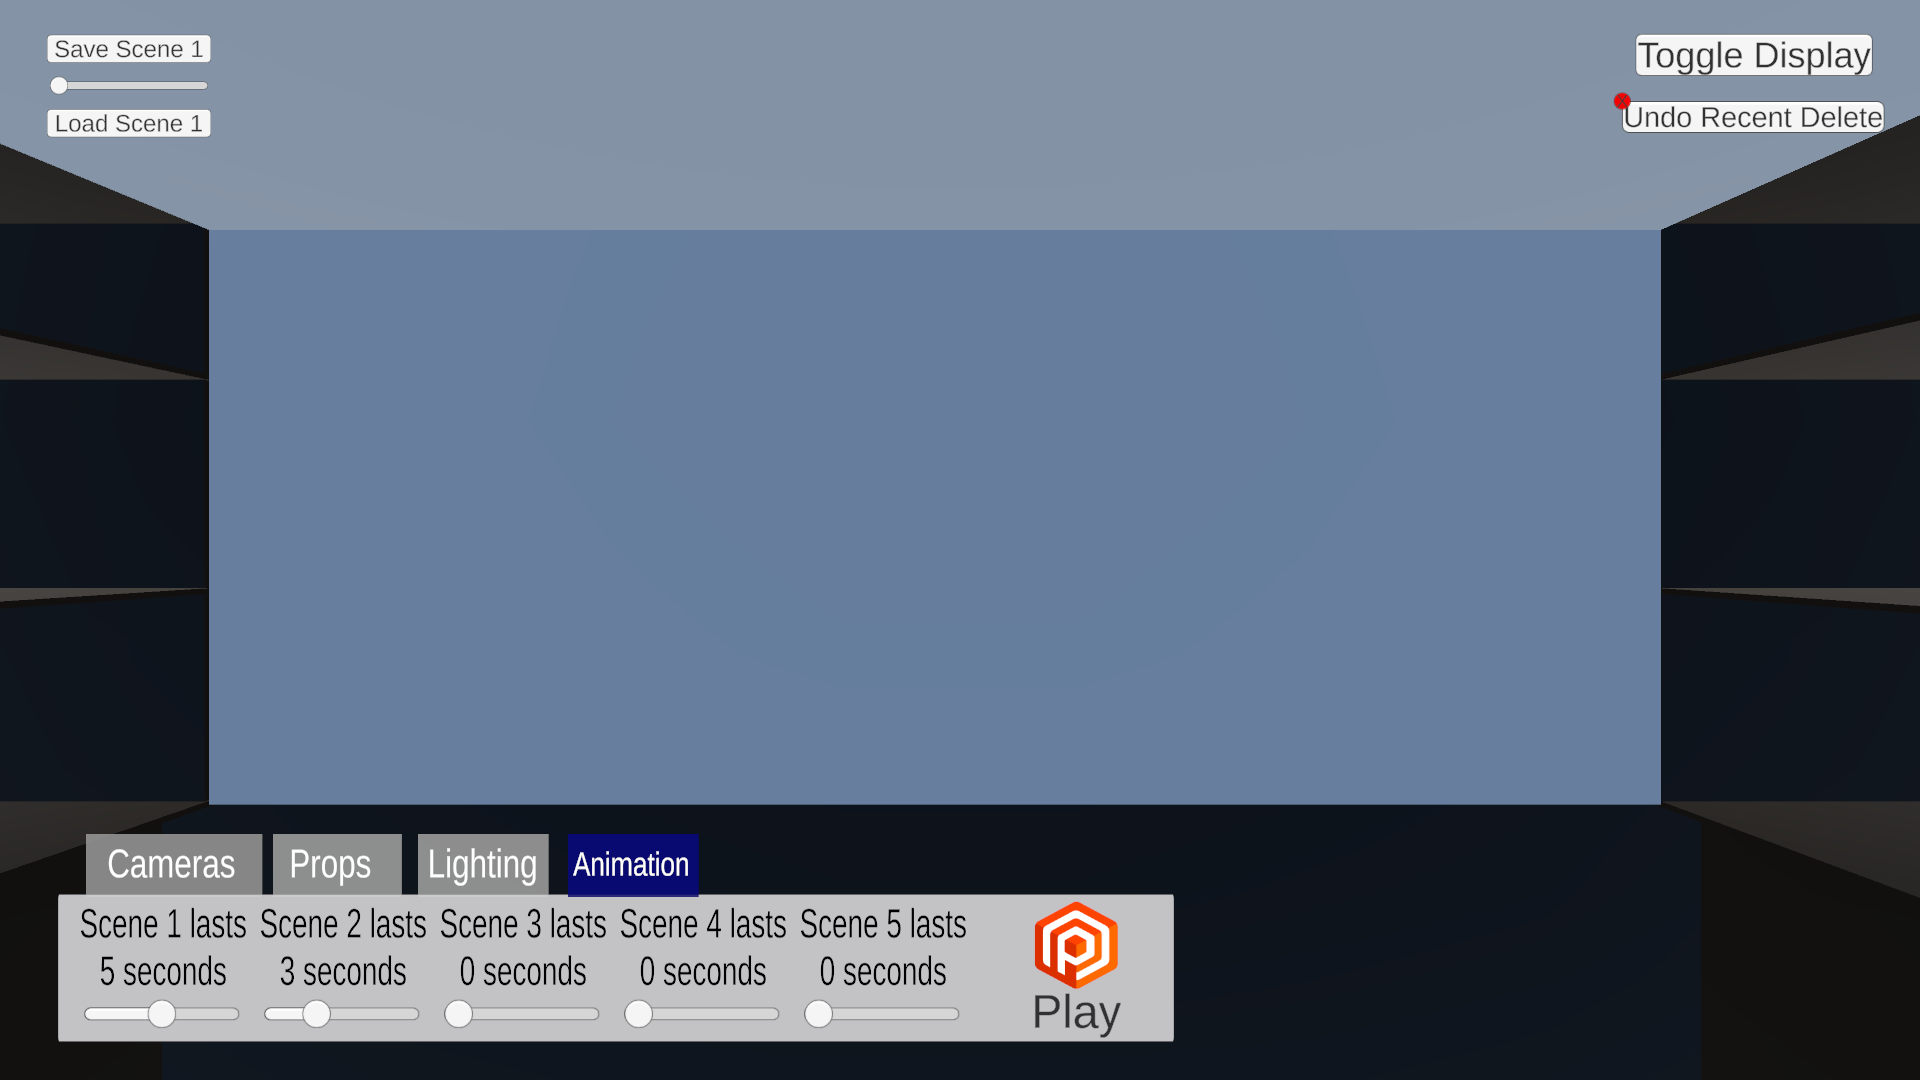
\includegraphics[width=.75\linewidth]{timeline.png}
\centering
    \caption{
        View of the animation timeline menu.
    }
    \label{fig:Fig4}
\end{figure}

\begin{figure}
    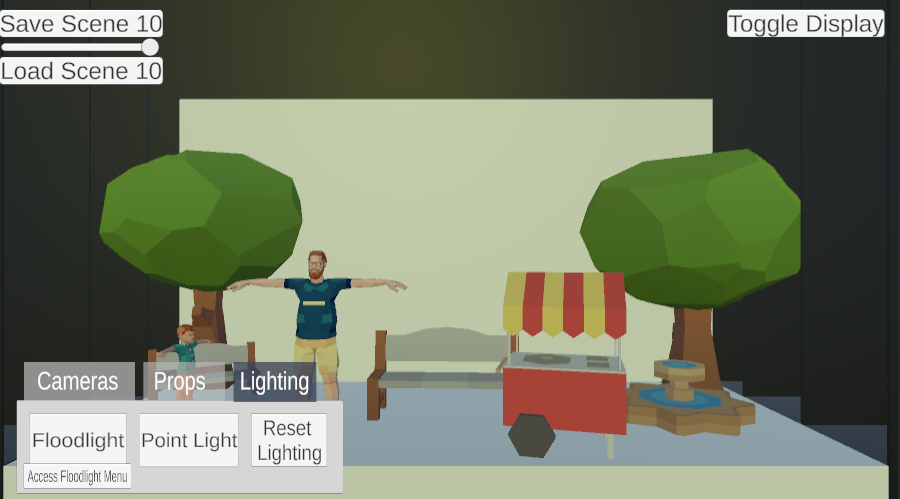
\includegraphics[width=.75\linewidth]{fullscene.png}
\centering
    \caption{
        Example of a full scene made in the software.
    }
    \label{fig:Fig5}
\end{figure}

\section{References}
\begin{hangparas}{.25in}{1}
Altieri, Alex. n.d. “Getting Started with Vectorworks Architect | What You Need to Know.” Blog.vectorworks.net. https://blog.vectorworks.net/getting-started-with-vectorworks-architect-what-you-need-to-know.

Creely, Edwin, and Danah Henriksen. Creativity and Digital Technologies. 1 Sept. 2019, pp. 1–6, https://doi.org/10.1007/978-981-13-2262-4143-1.

Dow Schull, Natasha. “The Folly of Technological Solutionism: An Interview with Evgeny Morozov.” Public Books, 9 Sept. 2013, www.publicbooks.org/the-folly-of-technological-solutionism-an-interview-with-evgeny-morozov/.

Gavin, Brady. 2018. “What Is Sketchup (and How Do I Use It)?” How-to Geek. How-To Geek. September 4, 2018. https://www.howtogeek.com/364232/what-is-sketchup/.

“Isometric Projection in Game Development.” n.d. Pikuma.com. https://pikuma.com/blog/isometric-projection-in-games.

Kittner, Elizabeth. “The Ethics of DEI: Cultivating a Positive Workplace.” Www.icpas.org, 2023, www.icpas.org/information/copy-desk/insight/article/fall-2023/the-ethics-of-dei-cultivating-a-positive-workplace.

STACBOND. 2020. “What Is AutoCAD and What Is It For, Software for Architecture and Engineering.” STACBOND. July 16, 2020. https://stacbond.com/en/what-is-autocad-and-what-is-it-for/.

“Vectorworks Basics — ArchiDabble | Architecture Resource Platform, CAD Packs, Portfolio Markups + More Services.” n.d. ArchiDabble. Accessed May 10, 2024. https://www.archidabble.com/tutorials/vectorworks-basics.

“Virtual Architect Home Design Software | Virtual Architect.” n.d. Www.homedesignsoftware.tv. Accessed May 10, 2024. https://www.homedesignsoftware.tv/how-to-videos/.
\end{hangparas}

\end{document}